\documentclass[conference]{IEEEtran}
\usepackage{amsmath,amssymb,booktabs,array}
\usepackage{graphicx}
\usepackage[hidelinks]{hyperref}
\usepackage{tikz}
\usetikzlibrary{arrows.meta,positioning}
\newcommand{\tool}{eGraphMap}
\newcommand{\eg}{e-graph}
\newcommand{\egs}{e-graphs}
\title{Technology Mapping over E-Graphs\protect\\with Delay-Constrained Area Recovery}
\author{\IEEEauthorblockN{Anonymous Authors}}
\begin{document}
\maketitle
\begin{abstract}
Technology mapping must choose a realizable circuit from equivalent Boolean structures while accounting for shared logic and timing.
We present \tool, a prototype for single-output standard-cell mapping over an e-graph.
Structural and functional cuts expose alternatives; physical matches retain input phase, pin assignment and conditional care information.
Whole-cover recovery charges shared instances once and reduces actual area under a validated timing limit.
Conditional matches remain outside the exact equivalence relation.
Evaluation uses all 20 EPFL arithmetic/control circuits, one shared \texttt{resyn2} input per design, and 47 supplied single-output ASAP7 cells.
A revised protocol limits total mapping time to 600 seconds and removes the earlier configurable node, pool, cut-count and iteration ceilings.
The full sweep returns 11 complete optimized covers; the other 9 cases retain separately verified source implementations after mapping timeout.
The results expose candidate-generation costs and do not establish full-suite dominance over the original baseline algorithms.
\end{abstract}
\begin{IEEEkeywords}
technology mapping, equality saturation, shared logic, area recovery,
satisfiability don't-cares
\end{IEEEkeywords}

\section{Introduction}
The quality of a mapped circuit depends on both the available Boolean
structures and how their implementations share physical cells. A rewrite
that looks attractive as a tree may duplicate a shared cone. Even with
single-output cells, independent choices at different roots can lose
sharing across reconvergent paths. Reachability provides another
opportunity: assignments to a cut boundary that can never occur permit
matches that fail a fully specified truth-table comparison.

Equality saturation addresses structural commitment by recording many
equivalent expressions in an e-graph \cite{egg}. Recent synthesis work has
already used this representation for technology-aware rewriting,
structural exploration, and FPGA LUT remapping
\cite{esyn,emorphic,eqmap}. Multi-output standard-cell mapping also has
established algorithms \cite{emap}. Combining these techniques requires a mapping model that distinguishes
Boolean equivalence from physical sharing and from conditional matching.
We focus on single-output mapping, with multi-output cells retained as an extension.

The study combines three mechanisms. First, structural cuts and exact
functional-quotient boundaries are constructed over the retained e-graph,
rather than committing to one extracted Boolean network. Second, matching
retains input phase, pin-specific delay and conditional care information;
SDC matches remain outside the global equivalence relation. Third,
whole-cover recovery separates physical-instance activation from binding,
charges shared cells once, and protects an already visited seed while
reducing actual area under a validated delay bound. Explicit source
proofs accompany exchanged bindings. The implementation exports acyclic
netlists and checks primary-output equivalence independently. Joint-output
selection is retained as an extension.


Standard-cell evaluation uses single-output ASAP7 subsets; synthetic
libraries test multi-output mechanisms separately. All methods share the
preoptimized input and netlist evaluator. Synthetic cell advantages are
not attributed to the standard-cell results.

\section{Background and Related Work}
\subsection{Mapping and shared logic}
Cut-based mapping summarizes the function at a root in terms of a bounded
set of boundary signals. Matching assigns that function to a library cell
under input permutation and phase choices. DAG-aware area-flow and exact
local area recovery account for sharing more effectively than additive
tree costs. The versatile mapping approach implemented in mockturtle
provides an important standard-cell baseline \cite{versatile}.

Calvino and De Micheli address multi-output matching and whole-network
optimization \cite{emap}. We retain e-graph alternatives and conditional
matches during candidate generation; emap receives the same library/input.

\subsection{Equality saturation in synthesis}
E-Syn introduces technology-aware costs for Boolean e-graph rewriting
\cite{esyn}. E-morphic scales structural exploration before mapping using
pruning and extraction techniques \cite{emorphic}. We evaluate both methods after a common front end. E-Syn uses a bounded
search with frozen cost models; E-morphic uses its final simulated-annealing
extractor. Their library restrictions and evaluation settings are specified
in Section~V.

EqMap uses e-graphs for FPGA LUT remapping \cite{eqmap}, optimizing LUT
count and depth. We evaluate a cross-target composition by flattening its
LUT network and applying a standard-cell backend. A control with the same
LUT conversion and backend isolates the effect of remapping. These results
measure the composition rather than native FPGA resource utilization.

Churchroad combines equality saturation with program synthesis for
target-specific FPGA primitives \cite{churchroad}. Its DSP-oriented target
differs from the standard-cell libraries considered here.

\section{Problem Formulation}
Let $G$ be a combinational Boolean network with primary inputs $P$ and
primary outputs $R$, and let $\mathcal{L}$ be a library. A physical library
cell $g$ has area $a_g$, a common input-pin set $I_g$, and output-pin
functions $f_{g,p}$. Its delay model contains input-to-output block delays
$d_{g,p,j}$ for functionally dependent inputs $j$.
We seek a finite acyclic implementation equivalent to $G$ on every primary
input assignment. We compare two lexicographic objectives:
\begin{equation}
  \min_{\rm lex}(A,D)\quad\text{or}\quad\min_{\rm lex}(D,A),\qquad
  A=\sum_{m\in\mathcal{M}}a_m x_m,
  \label{eq:objective}
\end{equation}
optionally subject to $D\leq D_{\max}$. Here $x_m$ selects a physical
candidate instance. Area and delay use the supplied genlib units.
The primary metric is minimized first; the secondary metric breaks ties
within numerical tolerance. No external target clock is imposed; internal area recovery instead fixes
the delay of its validated reference cover.
For integer extraction, a second solve constrains the best known primary
value and minimizes the secondary metric within the remaining time budget.
Lexicographic optimality is certified only if both stages prove optimality
and their extracted covers pass validation; a timeout preserves the best
checked cover without that certificate. Heuristic acceptance uses the same
priority order, but does not guarantee optimality. A lexicographic win is
reported separately from simultaneous Pareto improvement.

Each e-class denotes an exact Boolean equivalence class. A signal combines
an e-class identifier and a phase bit, permitting explicit inverted signals
and materialized inverter costs. A cut $C=(B,F)$ has an ordered boundary
$B$ and a truth table $F$ with $|B|\leq K$. Candidate $m$ specifies a cell,
a common assignment of physical inputs to boundary signals, and one or
more admissible bindings $(m,p,s)$ between output pin $p$ and target signal
$s$. Multiple targets of the same pin share a physical net when selected.
Output pins may remain unbound.

\section{Proposed Method}
\begin{figure}[t]
\centering
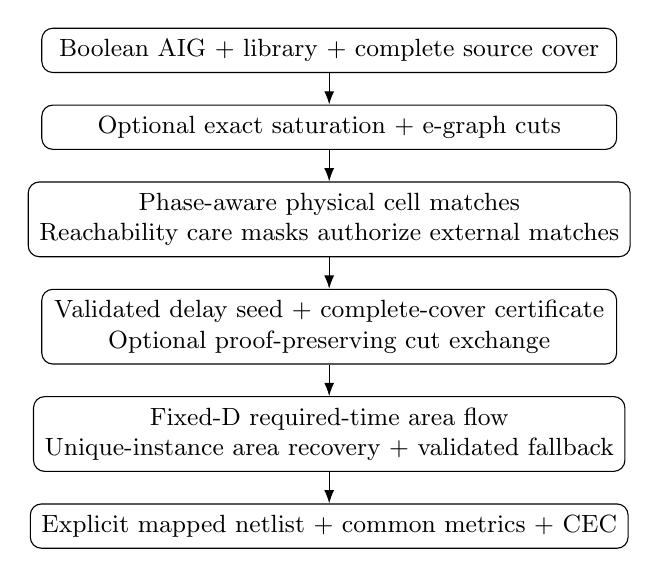
\begin{tikzpicture}[node distance=4mm,>=Latex,
 box/.style={draw,rounded corners,align=center,font=\small,
 minimum width=7.3cm,inner sep=4pt}]
\node[box] (a) {Boolean AIG + library + complete source cover};
\node[box,below=of a] (b) {Optional exact saturation + e-graph cuts};
\node[box,below=of b] (c) {Phase-aware physical cell matches\\
Reachability care masks authorize external matches};
\node[box,below=of c] (d) {Validated delay seed + complete-cover certificate\\
Optional proof-preserving cut exchange};
\node[box,below=of d] (r) {Fixed-D required-time area flow\\
Unique-instance area recovery + validated fallback};
\node[box,below=of r] (e) {Explicit mapped netlist + common metrics + CEC};
\draw[->] (a)--(b); \draw[->] (b)--(c); \draw[->] (c)--(d); \draw[->] (d)--(r); \draw[->] (r)--(e);
\end{tikzpicture}
\caption{Implementation flow. Conditional matches do not add equalities
to the exact e-graph.}
\label{fig:flow}
\end{figure}

\subsection{Cuts over exact alternatives}
The importer hash-conses Boolean operators and exact XOR/three-input truth-table contractions into one e-graph.
All original source helpers are retained in the time-only profile; compressed operators are not assumed to expose every AIG rewrite pattern.
Canonical e-classes support cut construction over alternative e-nodes.
Child boundaries are merged and their functions composed. Structural witnesses preserve a finite original implementation; cyclic e-graph alternatives do not permit cyclic physical covers.
Region ownership preserves complete physical boundaries and global target identifiers. It does not create separate per-region budgets.

The current policy removes configurable global count ceilings, rather than proving exhaustive enumeration. The algorithm still restricts the families of structures considered.
Small cuts use truth tables on actual support of at most six signals.
Seven-to-nine-input cells use directed structural matching, without constructing a table at the maximum library width for every cut.
Functional quotients use an existing class for $G(T)$ to form
$F(S)=Q(S\setminus T,G(T))$ only when all assignments uniquely determine every quotient entry.
The current proposal generator considers small quotient families, with fixed partner/batch rules. Safe exchange likewise uses a finite transaction batch; these algorithmic restrictions remain distinct from the removed global node and retained-pool ceilings.

Exact Not edges identify physical signal aliases; raw logical cut banks and physical pin interfaces remain explicit. Conditional matches establish no aliases.
Generation deduplicates physical instances before recovery. Delay-frontier propagation uses dependency notifications rather than repeated unchanged sweeps.
No optimality claim extends beyond the finite candidate problem actually constructed.

\subsection{Physical cell matching}
For each cut function, matching enumerates legal input permutations and
phases using the cell truth table and its physical pin delays. The
physical interface is kept explicit: two assignments with equal Boolean
functions can have different delay arcs. A single-output instance can
serve several equivalent targets or fanouts, but its area is charged only
once. Functionally independent pins contribute connectivity requirements
without contributing timing arcs. Each admitted binding retains its generating
boundary, care mask, target phase and physical pin assignment. Deduplication
merges proofs rather than discarding them. These records are local to one
mapping invocation; conditional care never licenses an e-class union.

Joint-output cells are an extension of this representation. Records with
the same physical cell name share an input assignment and one area charge,
while retaining separate output functions and delay vectors. Bounded
unions of neighboring or shared-leaf boundaries admit different output
supports; they do not exhaust all possible boundary unions. Full-adder
and disjoint-support synthetic tests exercise joint selection, open unused
pins and shared-instance accounting. The realistic inventories evaluated
here contain no multi-output cells.

\subsection{Conservative satisfiability don't-cares}
For a boundary $B=(b_1,\ldots,b_k)$, define the reachable image
\begin{equation}
 \mathcal{R}_B=\{(b_1(u),\ldots,b_k(u)):u\in\{0,1\}^{|P|}\}.
\end{equation}
A candidate output function $H$ may bind to target $F$ if
\begin{equation}
 (F\oplus H)\land C_B=0,\qquad \mathcal{R}_B\subseteq C_B,
 \label{eq:care}
\end{equation}
where $C_B$ is interpreted as a bit mask of care assignments. The prototype
traces the original boundary cones and enumerates their combined primary
input support only when both support and cone budgets permit. This yields
the exact reachable image for those bounded cases. Otherwise it uses the
full care set, losing opportunities rather than admitting unsound matches.

Matches remain external: agreement on reachable values is not a generic
identity for independent boundary variables. For fixed $B(X)$,
Equation~\eqref{eq:care} proves $F(B(X))=H(B(X))$; a concrete proof-backed
union could be sound, but we choose external storage. We handle SDCs,
not ODCs, environmental assumptions or sequential reachable states.

\subsection{Acyclic cover extraction}
For each admissible output binding $(m,p,s)$ introduce a binary variable
$z_{m,p,s}$. Let $\mathcal{B}(s)$ be its producer bindings and define
$q_s=\sum_{(m,p,s)\in\mathcal{B}(s)}z_{m,p,s}$. Non-free signals satisfy
$0\leq q_s\leq1$, required roots satisfy $q_s=1$, and every binding obeys
$z_{m,p,s}\leq x_m$. A selected instance requires availability of every
non-free physical input $j$, with free signal set $\mathcal{F}$:
\begin{equation}
 x_m\leq q_j,\qquad j\in I_m\setminus\mathcal{F}.
\end{equation}
Constants and primary input signals are free. Complemented inputs require
their actual producers unless an explicit library match realizes them.

Continuous levels $\ell_s$ prevent cycles. For every bound output and
every common physical input,
\begin{equation}
 \ell_s\geq\ell_j+1-M_\ell(1-z_{m,p,s}).
 \label{eq:acyclic}
\end{equation}
These constraints apply to secondary output pins as well as the first.
Requiring all physical inputs is conservative when a pin is irrelevant
to the selected output, but ensures a realizable connected instance.

When timing participates in extraction, arrival variables $t_s$ satisfy
\begin{equation}
 t_s\geq t_j+d_{m,p,j}-M_t(1-z_{m,p,s})
\end{equation}
for functionally dependent inputs only. Primary input arrival is zero and
$D\geq t_r$ for each root $r$. The implementation bounds levels and
arrivals before choosing the big-$M$ constants. Independent metric
recomputation rejects cyclic, incomplete, fractional, or timing-infeasible
solutions; solver termination alone is insufficient.

\subsection{Recovery and safe fallback}
A validated finite witness initializes recovery. A dependency frontier
releases producers with available inputs and supplies an acyclic delay
cover. A witness already required for candidate retention may cross this
interface; index remapping and validation consume the same recovery
window. Reporting-only frontiers cannot seed the mapper.

Before exchanging cuts, we preserve the complete visited cover, including
noncritical shared dependencies. Its bindings must retain generator
proofs in the new bank. A borrowed preparation view copies only changed records within the current safe-exchange transaction family. The commit moves unchanged records.
Equal physical inputs, pin arcs and area, together with injective producer
renaming, preserve the saved DAG and metrics. Failed preparation leaves
the old pool untouched; disposal consumes the same global window.
Unfinished support indices are rejected rather than used partially.

Area flow propagates required times from a fixed validated delay limit.
Actual-area recovery charges unique physical instances and refreshes
labels after accepted changes. A separate archive retains eligible,
already-scored whole covers under delay-area order: an over-area fast
point cannot suppress a feasible intermediate. Final validation enforces
both seed limits. This extra area constraint neither reproduces another
pipeline's historical final cover nor proves global exact-area optimality.
A timeout carries no optimality certificate.

\subsection{Correctness scope}
Assume exact rewrites, truthful cell functions and care masks containing
the original reachable image. Topological induction over an acyclic
cover establishes each bound signal's original semantics using
Equation~\eqref{eq:care}, hence output equivalence. This does not justify
independent ODC replacements or unproved generic conditional identities.
Explicit cell models, Yosys flattening and named-port ABC CEC
\cite{abc} independently check emitted networks. Unknown outcomes,
missing tools, undriven nets and cycles fail; corrupted-output tests
exercise rejection.

\section{Experimental Evaluation}
\subsection{Protocol and scope}
The suite contains all 20 EPFL arithmetic/control circuits \cite{epfl}; MtM is not included.
Each method reuses the same named AIG after one fixed ABC \texttt{resyn2} sequence and a preparation CEC. No method repeats this front end.
The common inventory contains all 47 single-output records in the supplied ASAP7 genlib \cite{asap7}: 45 named physical cell types and two zero-area constants. Seven cells have seven to nine inputs. This is not the full foundry PDK.
Earlier three-/four-input inventory results are archived as historical studies and are not substituted into the current table.

The current per-design/method allowance is 600 seconds of accumulated mapping wall time. Our clock includes source construction, import, saturation, cuts, matching, recovery and export.
There is no separate native-process, stage, address-space, node, search-ratio, retained-pool, cut-count or iteration ceiling in this execution policy.
The existing candidate families and safe-exchange batch rules remain algorithmic restrictions, as described above. CBC is disabled.
External preparation, conversion, independent CEC and metric reporting are excluded. Algorithmic intermediate metrics and mapping feedback remain inside the corresponding mapping call.
Stage work does not obtain a renewed outer deadline. Process termination and output draining can add small wall-time overhead after the deadline; such cases remain failures.

Baseline algorithms, source commits, models and search objectives are unchanged. Comparisons include ABC map/map-a, independent emap in both modes, EqMap followed by same-library ABC amap with staging controls, frozen-model E-Syn and final native E-morphic SA.
Only necessary port adaptation, library-range adaptation and timing instrumentation are applied.
Completed observations are reused only when exact dependencies and CEC remain valid and a stored search-inclusive upper bound is below 600 seconds. Search durations are added to the previous mapping bound; overlap may be double-counted conservatively in adopted bounds. Original timing labels and policies remain in the data; these observations are not fresh 600-second runs.
EqMap and E-Syn observations from the earlier limited-search adapter are retained as history and are retested; completion alone does not show those search limits were nonbinding. Every original failure is retained.

New EqMap runs meter the actual ABC process inside the initial Yosys LUT conversion. That shared mapping prefix is charged once to each relevant downstream method; conversion is excluded.
Historical EqMap runtimes retain the enclosing-Yosys upper-bound label.
The600-second allowance includes mapping-driven rewriting, candidate generation, extraction and SA, as well as cell/LUT mapping. Pure format conversion, the shared resyn2 input preparation, independentCEC and metric reporting are excluded. CEC is recorded as a verdict, without a separate runtime column. Native search and nested ABC callbacks share an active-interval union clock, avoiding double charging. E-morphic retains its unseeded native winner without reselection using public metrics. The preceding mapping-calls-only cohort is archived separately; its interrupted div search is an operator policy transition, not a retroactive timeout.
The earlier adapter-imposed E-Syn/EqMap two-second, 20,000-node, 16-iteration limits are removed from this cohort. EqMap uses its existing time-only interface; E-Syn uses its existing resource environment controls with nonbinding counts. Neither algorithm, model, rewrite rule, objective nor native winner selection is modified or tuned. Author-coded method steps, such as the original E-morphic rewrite and SA schedule, remain intact and are disclosed separately from experimental watchdogs. Consequently identical external wall-time ceilings do not imply identical search trajectories.
Times are observed wall times on the same host, without CPU pinning; author parallel settings are retained. They do not establish an isolated or machine-independent runtime gain.

Physical area counts every emitted instance once. Delay is the maximum output arrival using the maximum rise/fall unloaded block delay for functionally dependent pins; load, slew and interconnect are omitted.
Every numeric current output has independent named-port CEC against the original AIG, using explicit functional cell models.
Verification-only normalization never supplies candidates or scores to mapping.
Proof reuse requires identical physical netlist bytes, semantic connectivity, original input and library hashes; it is marked separately from a fresh CEC run. Interrupted redundant checks remain in the raw record.
Source fallback has its own metrics and CEC record, but does not count as completed optimized coverage.
Manifests retain commands, parameters, source/input/library/binary hashes, netlists and failed logs.

\begin{table*}[!t]\centering\fontsize{7.0}{8.5}\selectfont
\setlength{\tabcolsep}{2.4pt}\renewcommand{\arraystretch}{1.0}
\caption{Full 47-cell single-output inventory, one uniform delay-area eGraphMap configuration. T is mapping seconds; $\leq$ marks an inherited conservative upper bound. F retains failed or source-only optimization status; P is pending. A failed optimizer's separately verified source metrics remain in the data package. Reused completed baseline groups retain their original timing policy.}
\label{tab:epfl600}\begin{tabular}{l*{18}{r}}\toprule
Design & \multicolumn{3}{c}{ABC map} & \multicolumn{3}{c}{emap} & \multicolumn{3}{c}{EqMap} & \multicolumn{3}{c}{E-Syn} & \multicolumn{3}{c}{E-morphic} & \multicolumn{3}{c}{\tool} \\
 & A & D & T & A & D & T & A & D & T & A & D & T & A & D & T & A & D & T \\ \midrule
adder & 92.42 & 2574.36 & 0.06 & 90.29 & 2569.15 & 0.12 & 166.52 & 6388.99 & 35.04 & P & P & -- & 85.36 & 2340.21 & 31.99 & 87.06 & 2569.15 & 9.20 \\
bar & 285.88 & 171.90 & 0.14 & 188.56 & 170.48 & 0.14 & P & P & -- & P & P & -- & 245.19 & 175.52 & 47.49 & 262.77 & 168.29 & 12.66 \\
div & 3570.09 & 43089.85 & 1.94 & 3039.37 & 43095.86 & 1.29 & P & P & -- & P & P & -- & P & P & -- & F & F & 600.11 \\
hyp & 16009.92 & 196123.11 & 12.09 & 15147.22 & 195229.48 & 7.54 & P & P & -- & P & P & -- & P & P & -- & F & F & 600.03 \\
log2 & 1926.40 & 3984.94 & 2.72 & 1775.20 & 3864.80 & 1.51 & P & P & -- & P & P & -- & P & P & -- & F & F & 600.10 \\
max & 223.39 & 2076.07 & 0.18 & 181.01 & 2075.31 & 0.14 & P & P & -- & P & P & -- & 199.80 & 1653.93 & 71.88 & 209.68 & 2074.58 & 60.99 \\
multiplier & 1816.04 & 2662.96 & 1.40 & 1615.65 & 2630.33 & 0.88 & P & P & -- & P & P & -- & P & P & -- & F & F & 600.10 \\
sin & 411.86 & 1826.84 & 0.52 & 410.94 & 1759.04 & 0.36 & P & P & -- & P & P & -- & P & P & -- & F & F & 600.10 \\
sqrt & 1622.63 & 46860.57 & 1.29 & 1509.79 & 46977.00 & 0.90 & P & P & -- & P & P & -- & P & P & -- & F & F & 600.10 \\
square & 1168.40 & 2509.14 & 0.85 & 1099.20 & 2493.62 & 0.64 & P & P & -- & P & P & -- & P & P & -- & F & F & 600.03 \\
arbiter & 766.68 & 898.75 & 0.95 & 766.32 & 898.75 & 0.80 & P & P & -- & P & P & -- & P & P & -- & 766.62 & 898.75 & 119.75 \\
cavlc & 39.84 & 186.01 & 0.07 & 36.50 & 185.19 & 0.10 & P & P & -- & P & P & -- & 40.46 & 184.72 & 30.12 & 37.12 & 185.87 & 23.02 \\
ctrl & 6.89 & 103.17 & 0.05 & 6.60 & 103.17 & 0.10 & P & P & -- & P & P & -- & 7.17 & 91.38 & 20.40 & 6.70 & 103.17 & 2.05 \\
dec & 30.83 & 65.72 & 0.08 & 27.44 & 66.15 & 0.11 & 38.62 & 96.73 & 14.85 & P & P & -- & 34.14 & 80.64 & 23.17 & 30.83 & 65.72 & 4.86 \\
i2c & 71.14 & 165.79 & 0.10 & 66.11 & 166.44 & 0.12 & P & P & -- & P & P & -- & 68.89 & 144.08 & 40.38 & 69.00 & 165.79 & 22.13 \\
int2float & 12.98 & 181.00 & 0.05 & 11.49 & 181.00 & 0.10 & P & P & -- & P & P & -- & 14.22 & 136.36 & 21.85 & 12.33 & 181.00 & 2.10 \\
mem\_ctrl & 2665.27 & 1072.47 & 2.02 & 2348.96 & 1077.61 & 1.80 & P & P & -- & P & P & -- & P & P & -- & F & F & 600.03 \\
priority & 63.75 & 2045.58 & 0.08 & 60.30 & 2045.58 & 0.13 & P & P & -- & P & P & -- & 69.84 & 1006.42 & 55.73 & 64.46 & 2045.58 & 5.62 \\
router & 11.84 & 187.47 & 0.06 & 13.82 & 187.47 & 0.10 & P & P & -- & P & P & -- & 13.80 & 167.57 & 25.83 & 12.39 & 187.47 & 2.30 \\
voter & 986.05 & 718.25 & 0.59 & 956.17 & 655.18 & 0.60 & P & P & -- & P & P & -- & P & P & -- & F & F & 600.10 \\
\bottomrule\end{tabular}\vspace{1ex}
\centering\footnotesize
\setlength{\tabcolsep}{2.5pt}
\caption{Historical independent removals under the fixed 20,000-node profile, both inventories; these are not ablations of the current 600-second profile. A/D counts are lower/equal/higher for the ablated setting among jointly legal full-suite pairs. Repeated CEC is out of 18 attempts per setting; repeated A/D use same-round jointly legal pairs. Failure coverage is retained, not folded into PPA counts. T is the median mapping-process wall upper bound (seconds) over successful full-suite runs, excluding external preparation, CEC and evaluation.}
\label{tab:ablation}
\begin{tabular}{lrrrrrrr}\toprule
Setting & CEC/40 & A & D & T & Repeat CEC/18 & Repeat A & Repeat D \\ \midrule
Full configuration & 34/40 & -- & -- & $\leq$6.50 & 18/18 & -- & -- \\
No functional quotients & 34/40 & 16/6/12 & 1/25/8 & $\leq$5.86 & 18/18 & 6/3/9 & 3/9/6 \\
One-witness structural cuts & 34/40 & 5/18/11 & 0/34/0 & $\leq$6.45 & 18/18 & 5/8/5 & 0/18/0 \\
No input-phase matching & 22/40 & 11/2/9 & 0/2/20 & $\leq$1.52 & 12/18 & 12/0/0 & 0/0/12 \\
Canonical pin assignment & 28/40 & 16/1/11 & 0/0/28 & $\leq$1.86 & 12/18 & 12/0/0 & 0/0/12 \\
No SDC matching & 34/40 & 6/14/14 & 0/34/0 & $\leq$5.81 & 18/18 & 4/8/6 & 0/18/0 \\
No post-phase area recovery & 34/40 & 0/2/32 & 0/34/0 & $\leq$5.49 & 18/18 & 0/0/18 & 0/18/0 \\
No seed-metric protection & 34/40 & 3/22/9 & 0/34/0 & $\leq$6.44 & 18/18 & 5/7/6 & 0/18/0 \\
\bottomrule\end{tabular}\end{table*}\subsection{Measured coverage and limitations}
All 20 eGraphMap cases were attempted: 20 emitted outputs pass independent verification and 11 return complete optimized covers. The baseline checkpoint contains 36 of 120 groups and 102 qualified method observations out of 260 slots. Pending slots remain explicit. Attempted coverage is not equivalent to valid PPA coverage. Table~\ref{tab:epfl600} uses the first observation for each fixed configuration, never a best repetition or a per-design profile choice. Area-oriented baselines and all staging controls remain in the machine-readable full-scope gates.

Hyp does not return a complete optimized cover under the current policy; any verified source fallback remains separate. Log2 does not return a complete optimized cover under the current policy; any verified source fallback remains separate. Full-scope delay-area, area-delay and Pareto gates remain false. A strict delay improvement is a lexicographic win even if area increases; it is not simultaneous Pareto dominance.


\subsection{Unfinished runs}
Seven timeouts occur before cut construction finishes; two reach recovery.
All nine complete import; their native saturation spans are at most 1.25 seconds.
Div spends 464.79 seconds in cuts and 123.47 seconds in small-cell generation; recovery begins 597.04 seconds after import completion.
Mem\_ctrl reaches recovery 311.02 seconds after import, with 16.31 million retained instances versus div's 10.59 million.
Completed round spans grow to 135.81 seconds in hyp and 181.93 seconds in log2; sin also fails with only 5,085 imported e-nodes.
Per-round populations, RSS and inner recovery timings were not captured, preventing finer attribution or an out-of-memory diagnosis.
The traces motivate incremental cut/match/recovery work and publication of validated incumbents under one absolute clock.

\subsection{Baseline interpretation}
EqMap retains original six-input LUT remapping before standard-cell mapping; these results measure a cross-target composition, not native LUT utilization.
E-Syn retains original DAG features, frozen models and up to 30 ranked candidates. Its input conversion, candidate indexing and full-library calibration limit interpretation; no optimized feature/index probe enters this table.
E-morphic uses five rewriting iterations, ten initial samples and six rounds of ten neighbors at probability 0.8. Its feedback Liberty names the same physical cells, but loaded feedback delay differs from public unloaded delay.
Native exits, conversion failures, mapping timeouts and unproved CEC remain separate in the data package.

\subsection{Historical independent removals}
The earlier fixed-20,000-node study is retained in Table~\ref{tab:ablation}; it is not a same-binary ablation of the current 600-second policy or 47-cell inventory.
Functional quotients, witness-only cuts, input-phase matching, pin assignment, SDC, post-phase area recovery and seed protection were removed independently.
Area and delay counts use jointly legal pairs; failed coverage remains separate. The targeted repetitions use sqrt, sin and priority across both historical inventories, with alternating case order and rotated settings.
They neither establish full-suite stability nor isolate the later compact representation and timing-policy changes.


\section{Discussion and Conclusion}
Completing import and verifying a source implementation do not establish optimized mapping.
This sweep exposes substantial cut-construction and recovery costs after short native saturation spans.
Incremental construction and publication of validated incumbents are promising next steps, rather than demonstrated solutions.
Shared-instance accounting avoids double charging but does not prove globally minimum area.
Conservative SDC does not cover ODC or sequential reachability, and directed wide matching remains incomplete.
The completed covers and unfinished original-baseline comparison establish neither full-suite dominance nor repeatability.
Complete same-policy ablations, repetitions and CEC-verified measurements remain necessary before promoting this research configuration.

\clearpage
\twocolumn
\begin{thebibliography}{10}
\bibitem{egg} M. Willsey, C. Nandi, Y. R. Wang, O. Flatt, Z. Tatlock, and
P. Panchekha, ``egg: Fast and extensible equality saturation,''
\emph{Proc. ACM Program. Lang.}, vol. 5, POPL, art. 23, 2021.
\bibitem{emap} A. Tempia Calvino and G. De Micheli, ``Technology mapping
using multi-output library cells,'' in \emph{ICCAD}, 2023, pp. 1--9,
doi: 10.1109/ICCAD57390.2023.10323999.
\bibitem{versatile} A. Tempia Calvino, H. Riener, S. Rai, A. Kumar, and
G. De Micheli, ``A versatile mapping approach for technology mapping and
graph optimization,'' in \emph{ASP-DAC}, 2022, pp. 410--416.
\bibitem{esyn} C. Chen, G. Hu, D. Zuo, C. Yu, Y. Ma, and H. Zhang,
``E-Syn: E-graph rewriting with technology-aware cost functions for logic
synthesis,'' in \emph{DAC}, 2024, art. 124,
doi: 10.1145/3649329.3656246.
\bibitem{emorphic} C. Chen, G. Hu, C. Yu, Y. Ma, and H. Zhang,
``E-morphic: Scalable equality saturation for structural exploration in
logic synthesis,'' arXiv:2504.11574, 2025.
\bibitem{eqmap} M. Hofmann, B. Gokmen, and Z. Zhang,
``EqMap: FPGA LUT remapping using e-graphs,'' in \emph{ICCAD}, 2025,
pp. 1--9, doi: 10.1109/ICCAD66269.2025.11240672.
\bibitem{churchroad} G. Smith et al., ``Scaling program synthesis based
technology mapping with equality saturation,'' arXiv:2411.11036, 2024.
\bibitem{abc} R. Brayton and A. Mishchenko, ``ABC: An academic industrial-
strength verification tool,'' in \emph{CAV}, 2010, pp. 24--40.
\bibitem{asap7} L. T. Clark et al., ``ASAP7: A 7-nm FinFET predictive
process design kit,'' \emph{Microelectronics Journal}, vol. 53,
pp. 105--115, 2016.
\bibitem{epfl} L. Amar'u, P.-E. Gaillardon, and G. De Micheli, ``The EPFL combinational benchmark suite,'' in \emph{IWLS}, 2015.
\end{thebibliography}
\end{document}
